\documentclass[11pt,a4paper]{article}

\usepackage[utf8]{inputenc}
\usepackage[T1]{fontenc}
\usepackage{lmodern}
\usepackage{amsmath,amssymb}
\usepackage[table]{xcolor}
\usepackage{booktabs}
\usepackage{tabularx}
\usepackage{longtable}
\usepackage{xltabular}
\usepackage{caption}
\usepackage{array}
\usepackage{fancyhdr}
\usepackage{microtype}
\usepackage{etoolbox}
\usepackage{needspace}
\usepackage{float}
\usepackage{enumitem}
\usepackage{titlesec}
\usepackage{tikz}
\usetikzlibrary{arrows.meta,positioning,fit,backgrounds,calc}
\usepackage[a4paper, margin=1in, top=1.2in, bottom=1.2in, headheight=14pt]{geometry}
\usepackage[hidelinks]{hyperref}
\urlstyle{sf}
\makeatletter
\def\UrlFont{\sffamily}
\makeatother

% ---------------------------------------------------------
% Colours and small helpers
% ---------------------------------------------------------
\definecolor{navy}{HTML}{1F3A5F}
\definecolor{accent}{HTML}{2A7F9E}
\definecolor{softblue}{HTML}{EEF3F8}
\definecolor{softgrey}{HTML}{F5F6F8}
\definecolor{todo}{HTML}{A33A2A}

% Identifiers, paths and commands are set with \path, which breaks at slashes and
% underscores and stays in the sans-serif face (no monospace anywhere).
\DeclareUrlCommand\code{\urlstyle{sf}\def\UrlFont{\sffamily}}
\robustify\code
\newcommand{\cmd}[1]{{\sffamily\small #1}}
\newcommand{\fl}{-{}-}
\newcommand{\todo}[1]{\textcolor{todo}{[#1]}}
\newcommand{\hdr}[1]{\textbf{\color{white}\sffamily\small #1}}

\renewcommand{\arraystretch}{1.18}
\setlength{\tabcolsep}{5pt}
\newcolumntype{L}[1]{>{\raggedright\arraybackslash}p{#1}}
\newcolumntype{Y}{>{\raggedright\arraybackslash}X}

% Page style
\pagestyle{fancy}
\fancyhf{}
\fancyhead[L]{\small\sffamily\color{navy} Gamification and Experimentation Engine}
\fancyhead[R]{\small\sffamily\color{navy} Project Report --- Group 14}
\fancyfoot[C]{\small\thepage}
\renewcommand{\headrulewidth}{0.4pt}
\renewcommand{\headrule}{\hbox to\headwidth{\color{accent}\leaders\hrule height \headrulewidth\hfill}}
\renewcommand{\footrulewidth}{0pt}

% Headings
\titleformat{\section}{\Large\bfseries\sffamily\color{navy}}{\thesection}{0.7em}{}[{\color{accent}\titlerule[0.8pt]}]
\titleformat{\subsection}{\large\bfseries\sffamily\color{navy}}{\thesubsection}{0.6em}{}
\titleformat{\subsubsection}{\normalsize\bfseries\sffamily\color{accent}}{\thesubsubsection}{0.6em}{}
\titlespacing*{\section}{0pt}{1.6em}{0.9em}
\titlespacing*{\subsection}{0pt}{1.2em}{0.5em}

\setlength{\parindent}{0pt}
\setlength{\parskip}{0.55em}
\setlength{\emergencystretch}{3em}
\renewcommand{\_}{\textunderscore\allowbreak{}}
\setlist{itemsep=0.15em,topsep=0.3em}

\pretocmd{\section}{\Needspace{8\baselineskip}}{}{}
\pretocmd{\subsection}{\Needspace{7\baselineskip}}{}{}
\begin{document}

% ---------------------------------------------------------
% TITLE PAGE
% ---------------------------------------------------------
\begin{titlepage}
    \centering
    \vspace*{2.2cm}

    {\color{accent}\rule{\textwidth}{1.6pt}\par}
    \vspace{1.4em}
    {\sffamily\bfseries\fontsize{26}{30}\selectfont\color{navy} Project Report\par}
    \vspace{0.9em}
    {\sffamily\large\color{navy} Gamification, Social Cohort, Notification and\\[0.2em] Retention Experimentation Engine\par}
    \vspace{1.4em}
    {\color{accent}\rule{\textwidth}{1.6pt}\par}

    \vspace{2.2cm}

    {\large \textbf{Madhava Asrith}\par}
    {\normalsize AI23BTECH11007\par}
    \vspace{1.0cm}
    {\large \textbf{Sampadram}\par}
    {\normalsize AI23BTECH11025\par}

    \vspace{1.8cm}

    \begin{tabular}{r l}
        \textbf{Course} & CS5903 \\
        \textbf{Project} & Project 6 --- Group 14 \\
        \textbf{Repository} & \href{https://github.com/thisissam-1706/gamification-engine}{\sffamily github.com/thisissam-1706/gamification-engine} \\
        \textbf{Final tag} & \todo{tag, for example cs5903-final-2026} \\
        \textbf{Commit SHA} & \todo{full 40-character commit SHA} \\
    \end{tabular}

    \vfill
    {\normalsize November 2026\par}
    \vspace*{1.2cm}
\end{titlepage}

% ---------------------------------------------------------
% TABLE OF CONTENTS
% ---------------------------------------------------------
\pagenumbering{arabic}
\setcounter{page}{1}

\tableofcontents
\newpage

% ---------------------------------------------------------
% EXECUTIVE SUMMARY
% ---------------------------------------------------------
\section*{Executive Summary}
\addcontentsline{toc}{section}{Executive Summary}

Gamification features such as streaks, XP, leaderboards and reminders are only trustworthy if rewards can be reproduced, abuse is visible, notifications respect fatigue limits, and any claimed benefit comes from a controlled comparison. We built an event-sourced engine in Python (eventsourcing 9.5.5 on SQLite) that ingests validated learning events and keeps each learner's XP, streaks, freezes, quests and badges as a deterministic fold over an immutable log. On top of it sit weekly cohorts with a leaderboard, a rule-based remediation policy, a three-channel notification dispatcher, flag-only abuse detection, and an experiment pipeline for a streak-reminder trial (exp\_007).

All eight milestones (M1--M8) are implemented and all 18 acceptance tests pass; the engine test suite passed 1,333 of 1,333 tests in our final run. Replaying the log after wiping derived state reproduces identical results, for 15 learners (AT-15) and for a 1,000-learner, 114,974-event benchmark. Limitations: one process, synthetic data only, no built-in scheduler, simulated delivery channels, and abuse thresholds that are unvalidated.

% ---------------------------------------------------------
% 1. PROBLEM, SCOPE AND SUCCESS CRITERIA
% ---------------------------------------------------------
\section{Problem, Scope and Success Criteria}

\subsection{Users and actors}

\begin{xltabular}{\textwidth}{@{}L{3.3cm} Y@{}}
\rowcolor{navy} \hdr{Actor} & \hdr{Role in the system} \\
\endfirsthead
\rowcolor{navy} \hdr{Actor} & \hdr{Role in the system} \\
\endhead
\rowcolor{softgrey} Learner & Completes lessons, attempts checkpoint assessments, receives reminders and quest notices, and appears on a weekly leaderboard. \\
Learning service & The trusted producer (named \code{learning-svc} in the allow-list) of lesson, checkpoint and surface-view events. \\
\rowcolor{softgrey} Platform operator & Runs the engine tick and the experiment scripts, reads reports, and replays the log after a failure. \\
Analyst or instructor & Reads the experiment, abuse and leaderboard outputs to decide whether a policy helped. \\
\end{xltabular}

\subsection{Problem statement}

A learning platform that rewards activity has to answer four questions that simple counters cannot. Can a learner's score be explained and rebuilt after a failure? Can repeated or scripted activity be noticed without punishing honest learners? Can reminders be sent without exceeding a fatigue budget or ignoring consent? And can the platform tell whether a reminder policy actually improved learning rather than just activity? The literature we reviewed (Section~\ref{sec:related}) shows gamification effects are modest and depend on context, so we treat each of these as an engineering requirement and not as an assumption.

\subsection{Scope}

\begin{xltabular}{\textwidth}{@{}Y Y@{}}
\rowcolor{navy} \hdr{In scope} & \hdr{Out of scope} \\
\endfirsthead
\rowcolor{navy} \hdr{In scope} & \hdr{Out of scope} \\
\endhead
\rowcolor{softgrey} Canonical event ingestion, validation, deduplication and evidence (M1) & Real learner data; all data is synthetic \\
Deterministic XP, streaks, freezes, quests, badges, replay (M2) & Kafka/Redpanda, Redis and PostgreSQL (deferred, ADR-0005) \\
\rowcolor{softgrey} Weekly cohorts and SQLite-backed leaderboards (M3) & A learner-facing product or UI styling \\
Rule-based remediation quests (M4) & Adaptive or bandit allocation (ADR-0004) \\
\rowcolor{softgrey} In-app, simulated push and simulated email notifications (M5) & Real push or email providers \\
Flag-only abuse detection (M6) & ML anomaly detection, XP clawback, confirmed signals (ADR-0003, ADR-0006) \\
\rowcolor{softgrey} Fixed 50/50 experiment assignment, metrics, fatigue reporting (M7) & Claims of real-world causal effect \\
Full-state rebuild, latency, outage recovery, benchmark (M8) & Distributed deployment; the engine has no built-in scheduler \\
\end{xltabular}

\subsection{Assumptions and constraints}

\begin{itemize}
    \item The team has two members and an eight-week schedule, which drove the choice of a single-process design (ADR-0002, ADR-0005).
    \item Day boundaries use each learner's IANA time zone. Arrival time is the server's own receive clock, never a value from the event envelope.
    \item Events more than 72 hours late are rejected; the notification cap is 5 messages per learner per rolling 24 hours; quiet hours are 22:00--08:00 learner local time (\code{docs/problem-boundaries.md}).
    \item Cohort size bounds default to 500 and 5,000 members (\code{src/leaderboard/models.py}); small test populations override them.
    \item All evidence comes from synthetic workloads generated by \code{src/scale_and_recovery/workload.py} and \code{simulator/}.
\end{itemize}

\subsection{Approved milestones and frozen acceptance tests}

\begin{xltabular}{\textwidth}{@{}L{1.1cm} L{4.1cm} L{2.9cm} L{2.2cm} Y@{}}
\rowcolor{navy} \hdr{ID} & \hdr{Milestone} & \hdr{Acceptance tests} & \hdr{Owner} & \hdr{Peer reviewer} \\
\endfirsthead
\rowcolor{navy} \hdr{ID} & \hdr{Milestone} & \hdr{Acceptance tests} & \hdr{Owner} & \hdr{Peer reviewer} \\
\endhead
\rowcolor{softgrey} M1 & Canonical engagement events & AT-1 & Sampadram & Madhava Asrith \\
M2 & Deterministic gamification & AT-2, 3, 4, 5, 16 & Sampadram & Madhava Asrith \\
\rowcolor{softgrey} M3 & Cohorts and leaderboards & AT-7 & Madhava Asrith & Sampadram \\
M4 & Intervention and quest policy & AT-17 & Madhava Asrith & Sampadram \\
\rowcolor{softgrey} M5 & Multi-channel notifications & AT-8, 9, 10, 11, 14 & Madhava Asrith & Sampadram \\
M6 & Abuse detection & AT-6 & Sampadram & Madhava Asrith \\
\rowcolor{softgrey} M7 & Experimentation and metrics & AT-12, 13, 15 (partial), 18 & Sampadram & Madhava Asrith \\
M8 & Scale and recovery & AT-2, AT-15 & Madhava Asrith & Sampadram \\
\end{xltabular}

The wording of the 18 tests is kept in \code{docs/traceability-matrix.md} and is reproduced in Section~\ref{sec:matrix}.

\subsection{Done-when workflow and target metrics}

\textbf{Workflow.} A learner event arrives from the learning service, is validated and deduplicated, and is folded into the learner's state. The leaderboard, notifications and remediation then reflect it. If all derived state is wiped and rebuilt from the retained log, every learner's XP, streak count and freezes, and every leaderboard rank, match their pre-wipe values exactly. The experiment report can be regenerated from the stored log with identical output.

\begin{xltabular}{\textwidth}{@{}L{4.8cm} Y@{}}
\rowcolor{navy} \hdr{Target} & \hdr{Threshold} \\
\endfirsthead
\rowcolor{navy} \hdr{Target} & \hdr{Threshold} \\
\endhead
\rowcolor{softgrey} Replay determinism & Pre-wipe and post-rebuild checksums equal (AT-2, AT-15) \\
Leaderboard latency (update, top-k, surrounding, rank) & p50 $\le$ 5 ms, p95 $\le$ 20 ms, p99 $\le$ 50 ms \\
\rowcolor{softgrey} Notification outage recovery & Every routed proposal recovered, zero duplicate deliveries \\
Fatigue cap & No learner above 5 messages in any rolling 24 hours \\
\rowcolor{softgrey} Cohort gaming guardrail & Share of weekly XP from repeat completions at most 15\% \\
Assignment balance & Sample-ratio chi-square test with alpha 0.001 raises no alert \\
\rowcolor{softgrey} Primary experiment metric & Percent of eligible learners who pass their first eligible checkpoint within 14 days of assignment; missing outcomes count as not mastered \\
\end{xltabular}

% ---------------------------------------------------------
% 2. RELATED WORK
% ---------------------------------------------------------
\section{Related Work, Baselines and Alternatives}
\label{sec:related}

\subsection{Literature}

Hamari et al.\ reviewed 24 empirical studies and found mostly positive effects that depend on context and on the users \cite{hamari2014}. The meta-analysis by Sailer and Homner reports small positive effects on cognitive, motivational and behavioural outcomes, but the motivational and behavioural effects were less robust in higher-quality studies \cite{sailer2020}. For streaks specifically, Aulagnon et al.\ ran a randomised trial with about 60,000 students in Peru; streak messages and personalised reminders increased platform use, while the learning result rests on roughly 1,500 students who took an endline test \cite{aulagnon2025}. Yanez et al.\ used multi-armed bandits to choose reminder-email subject lines and observed that an adaptive policy can favour an arm even when no real difference exists \cite{yanez2022}. Bälter et al.\ found that personalised reminders improved timeliness by 14 percentage points in a study of only 39 adult learners \cite{balter2023}.

Four design decisions follow from this. We use fixed 50/50 assignment instead of a bandit (ADR-0004). The primary metric is checkpoint mastery and not opens or clicks. Fatigue and opt-outs are reported next to the benefit. And every claim from the simulator is limited to checking mechanisms, not real causality.

\subsection{Existing systems}

Duolingo is a closed product that uses streaks, leagues and reminders and states that it tests features with internal experiments; it is not a reusable backend. Funifier is a commercial gamification platform with a REST API, SDKs and configurable challenges. The FGPE gamification service is an open-source GraphQL service for programming education. From the public material we reviewed, none of them describes a versioned event model with deterministic replay and recovery, retroactive abuse detection with evidence references, or a controlled experiment that measures learning and fatigue together. We did not have source access to the first two, so this is a statement about their public documentation only.

\subsection{Alternatives considered}

\begin{xltabular}{\textwidth}{@{}L{2.5cm} L{3.4cm} L{3.4cm} Y@{}}
\rowcolor{navy} \hdr{Decision} & \hdr{Selected} & \hdr{Alternative} & \hdr{Why} \\
\endfirsthead
\rowcolor{navy} \hdr{Decision} & \hdr{Selected} & \hdr{Alternative} & \hdr{Why} \\
\endhead
\rowcolor{softgrey} State storage & eventsourcing library on SQLite, one process (ADR-0005) & PostgreSQL outbox (ADR-0001); Kafka/Redpanda with Redis (ADR-0002) & Gives ordered streams, aggregate rehydration and atomic saves without new infrastructure; distributed parts deferred until measurements justify them. \\
Abuse detection & Rule-based, retroactive, flag-only (ADR-0003, ADR-0006) & Real-time ML anomaly model & Auditable, replay-compatible, needs no labelled abuse data. \\
\rowcolor{softgrey} Allocation & Deterministic fixed 50/50 (ADR-0004) & Contextual bandit & Establishes a baseline first; propensity is still logged. \\
Repeat-XP decay & Part of the reward path, opt-in rule set v2 (ADR-0006) & Detection-only discount; clawback; editing v1 & A reward is decided once and stored; published rule sets stay immutable. \\
\rowcolor{softgrey} Remediation & Pure rule-based policy, decisions stored (ADR-0007) & Bandit policy; recompute on replay & Explainable and reproducible; a later rule change cannot rewrite history. \\
\end{xltabular}

\subsection{Reused frameworks and what we added}

\begin{xltabular}{\textwidth}{@{}L{3.7cm} L{2.2cm} L{2.4cm} Y@{}}
\rowcolor{navy} \hdr{Component} & \hdr{Version} & \hdr{Licence} & \hdr{Use} \\
\endfirsthead
\rowcolor{navy} \hdr{Component} & \hdr{Version} & \hdr{Licence} & \hdr{Use} \\
\endhead
\rowcolor{softgrey} eventsourcing & 9.5.5 (pinned) & BSD-3-Clause & Aggregates, event store, notification log \\
jsonschema & 4.26.0 (lockfile) & MIT & Draft-7 validation of event envelopes and payloads \\
\rowcolor{softgrey} pytest & 9.1.1 (lockfile) & MIT & Test runner (development) \\
PyYAML & 6.0.3 (installed) & MIT & Experiment definition check (development) \\
\rowcolor{softgrey} Python standard library & 3.11+ & PSF & sqlite3, zoneinfo, hashlib, importlib.resources \\
\end{xltabular}

The library gives us the event store and aggregate machinery. Everything above it is our own work: the learner aggregate and rules, ingestion with its evidence store, the cohort builder and leaderboard projection with reconciliation, the remediation policy, the notification dispatcher and guardrails, the abuse rules, the experiment runner and metrics, the rebuild and benchmark harnesses, and the simulator.

\subsection{Working baselines}

We compare against four baselines, each defined before measurement. For the reminder policy the baseline is the control arm (variant\_b), which receives no streak-risk reminders. For rewards it is rule set v1, which pays a flat 100 XP. For recovery it is the learner state read from the live aggregates immediately before the wipe. For leaderboard latency it is the fixed 5/20/50 ms threshold set.

\subsection{Methodology record}
\label{sec:method}

The original decisions (ADR-0001, ADR-0002 and ADR-0004) chose a Kafka/Redpanda and Redis event pipeline and made a contextual bandit the core allocation engine. After the Week 2 review we replaced the infrastructure plan with the eventsourcing library and SQLite (ADR-0005) and settled on fixed 50/50 assignment, with bandit allocation left as future work (changelog of ADR-0004). The methodology was therefore \emph{changed} from the original proposal.

% ---------------------------------------------------------
% 3. ARCHITECTURE
% ---------------------------------------------------------
\Needspace{12cm}
\section{Architecture and Implementation}

\subsection{Component and data flow}

\begin{figure}[H]
\centering
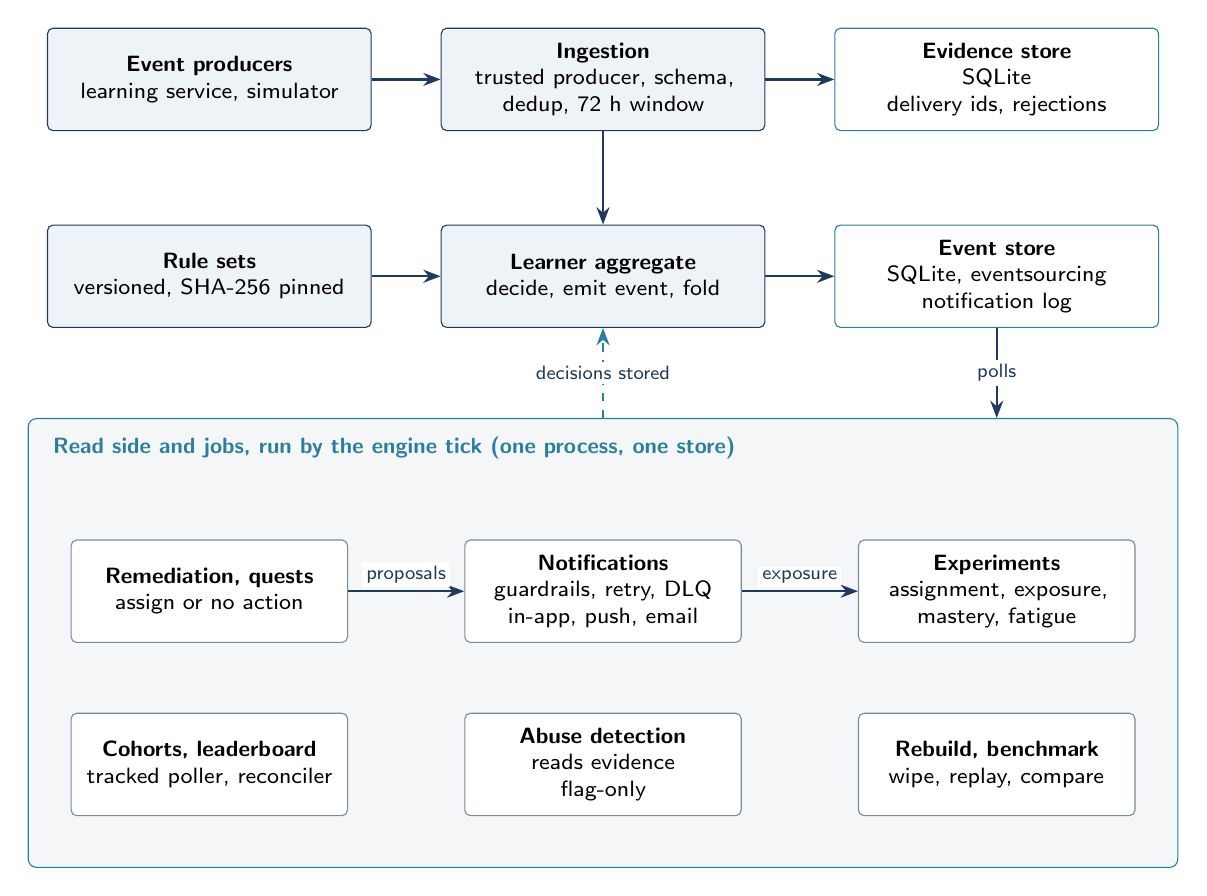
\begin{tikzpicture}[
    font=\sffamily\footnotesize,
    box/.style={draw=navy, fill=softblue, rounded corners=2pt, minimum height=1.3cm, align=center, inner sep=3pt, text width=3.9cm},
    store/.style={draw=accent, fill=white, rounded corners=2pt, minimum height=1.3cm, align=center, inner sep=3pt, text width=3.9cm},
    job/.style={draw=navy!60, fill=white, rounded corners=2pt, minimum height=1.3cm, align=center, inner sep=3pt, text width=3.3cm},
    arr/.style={-{Stealth[length=2.2mm]}, thick, color=navy},
    darr/.style={-{Stealth[length=2.2mm]}, thick, dashed, color=accent},
    lbl/.style={font=\sffamily\scriptsize, color=navy, fill=white, inner sep=1.5pt}
]
% write path
\node[box]   (prod)  at (0,0)     {\textbf{Event producers}\\learning service, simulator};
\node[box]   (ing)   at (5,0)     {\textbf{Ingestion}\\trusted producer, schema, dedup, 72 h window};
\node[store] (evd)   at (10,0)    {\textbf{Evidence store}\\SQLite\\delivery ids, rejections};
\node[box]   (rules) at (0,-2.5)  {\textbf{Rule sets}\\versioned, SHA-256 pinned};
\node[box]   (agg)   at (5,-2.5)  {\textbf{Learner aggregate}\\decide, emit event, fold};
\node[store] (log)   at (10,-2.5) {\textbf{Event store}\\SQLite, eventsourcing\\notification log};

% read side
\node[draw=accent, fill=softgrey, rounded corners=3pt, minimum width=14.6cm, minimum height=5.7cm,
      anchor=north] (rs) at (5,-4.3) {};
\node[font=\sffamily\footnotesize\bfseries, color=accent, anchor=north west] at ($(rs.north west)+(0.2,-0.12)$)
     {Read side and jobs, run by the engine tick (one process, one store)};
\node[job] (iv) at (0,-6.5)  {\textbf{Remediation, quests}\\assign or no action};
\node[job] (nt) at (5,-6.5)  {\textbf{Notifications}\\guardrails, retry, DLQ\\in-app, push, email};
\node[job] (ex) at (10,-6.5) {\textbf{Experiments}\\assignment, exposure,\\mastery, fatigue};
\node[job] (lb) at (0,-8.7)  {\textbf{Cohorts, leaderboard}\\tracked poller, reconciler};
\node[job] (ab) at (5,-8.7)  {\textbf{Abuse detection}\\reads evidence\\flag-only};
\node[job] (rb) at (10,-8.7) {\textbf{Rebuild, benchmark}\\wipe, replay, compare};

\draw[arr] (prod) -- (ing);
\draw[arr] (ing) -- (evd);
\draw[arr] (ing) -- (agg);
\draw[arr] (rules) -- (agg);
\draw[arr] (agg) -- (log);
\draw[arr] (log.south) -- (log.south |- rs.north) node[lbl, midway] {polls};
\draw[darr] (agg.south |- rs.north) -- (agg.south) node[lbl, midway] {decisions stored};
\draw[arr] (iv) -- (nt) node[lbl, midway, above=1pt] {proposals};
\draw[arr] (nt) -- (ex) node[lbl, midway, above=1pt] {exposure};
\end{tikzpicture}
\caption{Single-process architecture and the integrated flow reviewers asked for: a learning event is ingested, rewarded, ranked, checked for remediation, delivered under the notification guardrails, recorded as exposure and joined to the checkpoint outcome. The dashed arrow shows decisions being stored back on the learner aggregate.}
\label{fig:arch}
\end{figure}

\subsection{Major components}

\begin{xltabular}{\textwidth}{@{}L{3.0cm} Y L{3.6cm}@{}}
\rowcolor{navy} \hdr{Component} & \hdr{Responsibility and interface} & \hdr{Source} \\
\endfirsthead
\rowcolor{navy} \hdr{Component} & \hdr{Responsibility and interface} & \hdr{Source} \\
\endhead
\rowcolor{softgrey} Ingestion & Validates the envelope against Draft-7 schemas; checks producer against an allow-list; rejects reward fields in source events; deduplicates on \code{event_id:rule_version}; binds each event\_id permanently to one business action; rejects deliveries older than 72 h by server receive time; carries correlation and causation ids. & \code{src/ingestion/} \\
Learner aggregate & Public methods decide and emit events; event handlers only fold state. Covers lessons, checkpoint attempts, streaks, freezes, quests, badges, experiment assignment and exposure, remediation decisions, cohort assignment. & \code{src/state_machine/} \\
\rowcolor{softgrey} Rules & Immutable rule sets v1 (flat) and v2 (decay); the digest is checked on load. Streak calculation is a pure function of activity dates and freezes. & \code{src/state_machine/rules.py} \\
Cohorts and leaderboard & Weekly cohort builder; atomic admission; SQLite projection with a deterministic order (score descending, then time first reached, then subject id); poller; weekly cycle; differential reconciliation. & \code{src/leaderboard/} \\
\rowcolor{softgrey} Interventions & Pure policy \code{decide_remediation}; runner stores every decision; \code{remediation_v1} quest; expiry sweep; opt-in notification wrapper. & \code{src/interventions/} \\
Notifications & Dispatcher with consent, TTL, cap and quiet-hour guardrails; up to three delivery attempts; DLQ and replay; in-app, push and email adapters (the last two simulated); streak-risk reminder generator. & \code{src/notifications/} \\
\rowcolor{softgrey} Abuse detection & Detectors for replay, duplicate exploitation, impossible timing, scripted farming, receive timing and review misuse; cohort gaming report; signals stored with evidence references. & \code{src/abuse/} \\
Experiments & Hash assignment, eligibility and decision stores, mastery metric, exposure, fatigue, sample-ratio check, \code{run_experiment}. & \code{src/experiments/} \\
\rowcolor{softgrey} Scale and recovery & Rebuild harness, workload generator, latency measurement, outage harness, reproduction checks. & \code{src/scale_and_recovery/} \\
Simulator & Persona population, baseline stream, bounded perturbation, sensitivity sweep, pilot streams and report. & \code{simulator/} \\
\rowcolor{softgrey} Scripts & One-shot tick, experiment entry point, scale benchmark, cohort benchmark, evidence capture. & \code{scripts/} \\
\end{xltabular}

\subsection{M1: Event ingestion and contracts}

Every learner event enters through one validation path, and each step can reject it with a stored reason. The checks run in this order.

\begin{enumerate}[leftmargin=2em]
    \item \textbf{Schema and producer.} The envelope and payload are validated against Draft-7 schemas. The producer named in the envelope must match the authenticated producer of the call, and must be allowed to send that event type. The learning service may send lesson completions, checkpoint attempts and surface views; XP, streak, quest and badge events are reserved for the engine.
    \item \textbf{Reward fields.} A source event that carries \code{xp_amount}, \code{reward_id} or \code{new_streak} is rejected, so a producer cannot claim a reward.
    \item \textbf{Dedup key.} The expected key is $\text{event\_id}\,{:}\,\text{rule\_version}$, where the version comes from trusted configuration (or from the version the event was first accepted under, for a redelivery). A key built with any other version is rejected, so a producer cannot choose a more generous rule set.
    \item \textbf{Permanent binding.} Each event\_id is bound for good to the first business action it carried. A redelivery of an accepted event is answered from that binding, and the same event\_id with different content is rejected as a conflict. A re-sent business action under a new event\_id is dropped by its action id. Nothing expires, so a duplicate sent after the cache window still changes no XP.
    \item \textbf{Late window.} For an event with no binding yet, the lateness is $\Delta = t_{\text{receive}} - t_{\text{occurred}}$, where $t_{\text{receive}}$ is the server's own clock. An event with $\Delta$ above 72 hours is rejected. Because the binding is checked first, a redelivery of an accepted event is never rejected as late.
\end{enumerate}

Accepted and rejected deliveries are written to the evidence tables with their reason, so that the abuse detectors (M6) can read replay and resubmission patterns later. Correlation and causation ids are copied from the envelope to every event the engine derives from it, which makes any XP award traceable to the delivery that caused it.

\subsection{M2: Deterministic learner state}

\textbf{Decide, then fold.} Each public method on the learner aggregate checks the command against current state and, if allowed, emits an event; each event handler only updates fields. Replay runs the handlers alone, so no decision or reward is recomputed. This is why a rule change cannot alter a stored award (AT-5) and why a rebuild reproduces state exactly (AT-2, AT-15).

\textbf{XP.} For the $N$-th prior eligible completion of the same lesson ($N=0$ for the first), with base amount $E$:
\[
\text{xp}(N)=
\begin{cases}
E & \text{if no decay is configured or } N=0,\\[2pt]
\max\!\Big(0,\ \big\lfloor E\cdot p/100\big\rfloor - s\,(N-1)\Big) & \text{otherwise,}
\end{cases}
\]
where $p$ is \code{first_repeat_percent} and $s$ is \code{step_xp}. Rule set v1 has no decay and always pays $E=100$. Rule set v2 uses $p=50$ and $s=20$, so the awards for $N=0,1,2,3,4$ are $100, 50, 30, 10, 0$. Review and remediation completions are exempt from decay, which is why M6 also watches for misuse of that exemption.

\textbf{Rule-set integrity.} A rule set is a frozen record of $E$, the quest targets, the badge threshold and badge id (plus the decay pair for v2). Its digest is the SHA-256 of the key-sorted compact JSON of those fields, and the loader refuses a file whose stored digest does not match. Changing any value therefore needs a new version number and not an edit.

\textbf{Activity date and streaks.} The activity date is the event time converted to the learner's IANA time zone. Let the distinct activity dates be $d_1 < d_2 < \dots$ and let $m_i = (d_i - d_{i-1}) - 1$ be the number of missed days before $d_i$. The streak value $S_i$ follows
\[
S_i=
\begin{cases}
1 & i=1,\\
S_{i-1}+1 & m_i=0,\\
S_{i-1}+1 & m_i>0 \text{ and } F_i \ge m_i,\\
1 & m_i>0 \text{ and } F_i < m_i,
\end{cases}
\]
where $F_i$ is the number of unused freezes already acquired on or before $d_i$. When a gap is bridged, the $m_i$ earliest-acquired freezes are marked consumed. The function returns, for every date, the streak, the freezes remaining and the freezes consumed on that date. Because it is a pure function of the date set and the freeze records, a late event simply adds a date and the whole sequence is recomputed in chronological order (AT-3). Where the recomputed value differs from what was stored, the aggregate emits a revisioned streak event instead of rewriting history (AT-4).

\textbf{Badges and quests.} A badge qualifies when the badge id matches and $S \ge 7$ (rule set v1), and it is awarded at most once per learner, even if the streak breaks and returns to 7 (AT-16). The quest \code{lesson_starter_v1} completes after 3 lessons (its target in the rule set). Quest definitions for remediation live in a separate registry so that the rule-set digest does not change when quests are added.

\subsection{M3: Cohorts and leaderboard}

\textbf{Tier and module.} The builder reads only each learner's accepted lesson completions in the ISO week before the epoch. With $n$ prior-week lessons, the tier is casual for $n<3$, regular for $3 \le n < 10$ and intensive for $n \ge 10$. The learner's module is the most frequent text before the first slash of their lesson ids; ties go to the lexicographically smallest module and a learner with no usable prefix goes to \emph{general}. A learner whose latest lesson is at least 30 days before the reference time is excluded as inactive, while a learner with no history at all is treated as new. No demographic field is read.

\textbf{Bucketing and size limits.} Within each tier-and-module group, a learner's bucket is the first 8 bytes of $\text{SHA-256}(\text{JSON}[\text{subject}, \text{kind}, \text{tier or module}, \text{epoch}, \text{salt}])$ read big-endian, modulo the number of buckets. With automatic settings, a group of $g$ learners gets $\max(1,\ \lfloor g/(2\cdot \text{min\_size})\rfloor)$ buckets, so cohorts average about twice the minimum size. A group larger than the maximum is split into $k=\lceil g/\text{max\_size}\rceil$ equal parts (sizes differ by at most one). A new cohort below the minimum is merged into the nearest cohort that still has room, ranked by same tier, then same module, then lowest cohort id, and a cohort that fits nowhere stays as it is, so the maximum always holds. A learner who already has a cohort for the week is never moved.

\textbf{Atomic admission.} Reading the member count and inserting the membership run inside one \code{BEGIN IMMEDIATE} transaction, so two writers cannot both take the last seat.

\textbf{Score and order.} A learner's weekly score is the sum of the XP awards applied to the leaderboard for the epoch. The tie-break timestamp \code{first_reached_at} is the time at which the running total first reached the final total. Entries are ranked by
\[
\text{score}\ \downarrow,\quad \text{first\_reached\_at}\ \uparrow,\quad \text{subject\_id}\ \uparrow,
\]
which gives every learner a distinct, repeatable rank. The poller applies engine events in stream-offset order and stores the offset it has reached.

\textbf{Reconciliation.} For a scope (global or one cohort), the reconciler rebuilds a canonical table from the applied events up to a pinned offset: for each learner, the summed score and the \code{first_reached_at} defined above. It then compares this table with the projected rows and makes the smallest correction: insert a missing row, update a row whose score or tie timestamp differs (only if the row is not newer than the pin), and remove a row that has no support in the events. Each run stores an audit record with the counts of inserts, updates and deletes (AT-7).

\subsection{M4 and M5: Remediation and notifications}

\textbf{Remediation policy (M4).} The policy \code{decide_remediation} is a pure function of the attempt, the learner's earlier decisions and the current instant. Its checks run in a fixed order, and the first to apply decides:
\begin{enumerate}[leftmargin=2em]
    \item the attempt is not the learner's first for that assessment: \emph{no action};
    \item the attempt passed: \emph{no action};
    \item an \emph{assign} decision exists with $t_{\text{decision}} > t_{\text{now}} - 14\text{ days}$: \emph{no action};
    \item otherwise \emph{assign} the quest \code{remediation_v1} with deadline $t_{\text{now}} + 7\text{ days}$.
\end{enumerate}
The decision id is derived from the attempt id, so deciding twice yields the same record, and every outcome, including \emph{no action}, is stored. The expiry sweep closes an unfinished quest with \code{expired_at} equal to its deadline and not the sweep time, so the stored fact does not depend on when the job ran (AT-17).

\textbf{Notification guardrails (M5).} A proposal passes the following gates in order, and the result is stored whether it is sent or not.
\begin{itemize}
    \item \textbf{Consent.} A global opt-out, or an opt-out of the message category, stops the message with reason \code{opt_out} and no delivery attempt (AT-11).
    \item \textbf{Time to live.} A proposal older than its TTL (default 86,400 s) expires.
    \item \textbf{Fatigue cap.} Let $c$ be the number of messages already sent to the learner in the preceding rolling 24 hours, counted over all channels together. The message is blocked when $c \ge 5$ (AT-14).
    \item \textbf{Quiet hours.} If the learner's local time is in $[22{:}00,\ 08{:}00)$, the message is rescheduled to the next 08:00 local time, so a candidate at 23:10 in Asia/Kolkata moves to 08:00 the next day (AT-8). Local time comes from the IANA zone, so a daylight-saving change cannot shift the boundary.
\end{itemize}
Proposals are deduplicated by proposal id before any gate (AT-9). A transient provider failure is retried up to three times; a permanent failure goes straight to the dead-letter queue; a message that exhausts its retries also lands there and can be replayed (AT-10).

\textbf{Streak-risk reminders.} For a treatment learner who has a streak but has not been active today, up to four reminders are planned at local 20:00, 21:00, 21:30 and 21:45 (gaps of 60, 30 and 15 minutes). A reminder is only planned when a lesson today would actually extend the streak, which is tested by running the same streak function with today's date added and checking that the result is above 1. Learners with under three days of tenure, opted-out learners and learners with no stored preferences are excluded and the reason is stored. Only the latest due reminder per learner is passed to the dispatcher, so all the guardrails above still apply.

\subsection{M6: Abuse detection}

Detection is retroactive and flag-only. The detectors read completions and the ingestion evidence, and write signals that carry references to the evidence rows; they never change XP. The thresholds below are taken from the first abuse rule set, and the second rule set keeps all of them and adds three more checks.

\begin{xltabular}{\textwidth}{@{}L{2.9cm} Y@{}}
\rowcolor{navy} \hdr{Detector} & \hdr{Flag condition} \\
\endfirsthead
\rowcolor{navy} \hdr{Detector} & \hdr{Flag condition} \\
\endhead
\rowcolor{softgrey} Replay & At least 5 distinct redelivered event ids within 60 minutes, or any event id reused with different content. \\
Duplicate exploit & At least 3 distinct completions of the same action re-sent under new event ids within 60 minutes, or a reward field present in a source event. \\
\rowcolor{softgrey} Impossible timing & Three consecutive gaps shorter than the minimum (20 s for lessons and remediation, 10 s for reviews) that together fit in 10 minutes; or more than 20 completions within 10 minutes. \\
Scripted farming & At least 10 repeat completions ($N\ge1$) within 24 hours; or, in any sliding run of 12 completions, a coefficient of variation of the gaps $\sigma/\mu \le 0.05$ with mean gap of at least 1 s. Reviews and remediation are excluded. \\
\rowcolor{softgrey} Second rule set only & Review misuse (more than 3 exempt completions of one lesson within 24 hours, or exempt completions of 3 or more lessons never done as a lesson); receive-time burst (more than 40 completions within 10 minutes of server time); future-dated events (more than 5 minutes ahead, at least 3 times). \\
\end{xltabular}

The timing detectors use producer-claimed times, which is why the receive-time check exists. The cohort guardrail is separate and works per cohort and ISO week. Writing $R$ for repeat XP (awards with $N \ge 1$) and $T$ for total XP in the cohort, the cohort is flagged when $T>0$ and $R/T>0.15$. The comparison is made with exact fractions, so a share of exactly 15\% is not flagged (AT-6).

\subsection{M7: Experiments and metrics}

\textbf{Assignment.} For subject $u$ and experiment $e$, the bucket is
\[
b=\Big(\text{int}_{\text{BE}}\big(\text{SHA-256}(\text{JSON}[u,e])_{[0:8]}\big)\Big) \bmod 100,
\]
and the learner gets \emph{variant\_a} (the reminder arm) if $b<50$ and \emph{variant\_b} (control) otherwise, with propensity $0.5$. The hash scheme name \code{hash_v2} is stored on every assignment event, so a later change of scheme is visible in the log. Assignment is stored when it happens. Exposure is a separate event, recorded only when a treatment learner views the treatment surface, so a control learner can never be counted as exposed (AT-12, AT-13).

\textbf{Primary metric.} Let a learner be assigned at $t_a$. Their first eligible attempt is the earliest attempt, by time then attempt id, inside $[t_a,\ t_a+14\text{ days}]$. The learner is mastered if that attempt has exactly one matching completion that passed, and $t_a \le t_{\text{attempt}} \le t_{\text{completion}} \le t_a + 14\text{ days}$. Every other assigned learner whose window has closed falls into one of: failed, missing outcome (no attempt, no completion, a completion for another assessment, or one after the window), invalid ordering, or conflicting records. Learners whose window has not closed by the declared data cutoff are \emph{immature} and are left out of the denominator. The rate is
\[
\text{mastery rate}=\frac{\text{mastered}}{\text{assigned}-\text{immature}},
\]
so a learner with no outcome counts as not mastered and cannot help the treatment arm by silently dropping out.

\textbf{Sample-ratio check.} With $a$ learners in variant\_a and $b$ in variant\_b, $N=a+b$ and expected count $E=N/2$ in each arm:
\[
\chi^2=\sum_{k\in\{a,b\}}\frac{(o_k-E)^2}{E},\qquad p=\operatorname{erfc}\!\Big(\sqrt{\chi^2/2}\Big),
\]
which is the one-degree-of-freedom chi-square tail. An alert is raised when $p<0.001$. The same check is run on the assigned learners and on the eligible learners, and either one failing makes the run invalid.

\textbf{Fatigue and contrast.} Observation for each learner runs from assignment to the earlier of 14 days later and the data cutoff. Messages per learner per day is the number of delivered and provider-failed messages divided by the learner-days observed. The rolling maximum is the largest number of messages in any 24-hour window starting at one of the learner's message times; a learner above 5 is a cap breach. The 95\% interval for the difference of two rates is the Wald interval
\[
(\hat p_1-\hat p_0)\ \pm\ 1.96\sqrt{\frac{\hat p_1(1-\hat p_1)}{n_1}+\frac{\hat p_0(1-\hat p_0)}{n_0}},
\]
and a result is reported as conclusive only if the interval excludes zero. \code{run_experiment} marks a run invalid, and gives the reasons, instead of reporting a number when a cap breach in treatment, a gaming-share breach, either sample-ratio alert, missing eligibility records, no eligible learners, mixed assessment versions, or delivery over the cap is found.

\subsection{M8: Scale and recovery}

\textbf{Full-state rebuild.} The harness first records a checksum over every learner's XP, streak and freezes and every leaderboard rank, in a fixed order. It then closes the application and the leaderboard store, deletes the leaderboard database and its sidecar files, opens a new application on the retained events database and a new empty read model, replays from the first entry, and recomputes the checksum with the same function. The test passes only if the two SHA-256 digests are equal; it also asserts a rebuild time under 10 seconds and a rate above 100 events per second on the small fixture (AT-15).

\textbf{Latency.} Each leaderboard operation (update, top-$k$, surrounding ranks, rank lookup) is timed with a high-resolution performance counter over 500 samples (top-$k$ uses $k=50$). The reported p50, p95 and p99 are order statistics of those samples and are compared with the 5, 20 and 50 ms thresholds.

\textbf{Outage recovery.} A channel is made to fail so that every routed proposal ends in the dead-letter queue. The channel is then restored and the queue is replayed. The harness passes when every proposal is drained exactly once and no learner receives a duplicate, and it reports the number of messages per second.

\textbf{Reproduction.} The experiment report and the engine run are each computed twice from the same stored log and compared by digest, since both are pure functions of the log and of the explicit \cmd{\fl now} instant.

\subsection{Data stores and schemas}

All persistence is SQLite. The event store is managed by the eventsourcing library. Our own tables are: the learner projection and its staging table; \code{ingestion_evidence}, \code{accepted_deliveries} and \code{delivery_ids}; the leaderboard tables (entries, applied events, checkpoints, processed offsets, reconciliation audits, cohort definitions, completion times, pending awards); the notification tables (proposals, dispatches, suppressions, DLQ, rescheduled, guardrail violations); \code{experiment_eligibility} and \code{experiment_decisions}; and \code{abuse_signals}. Nineteen engine event schemas plus the envelope, cohort definition and leaderboard query and response schemas live in \code{src/schemas/}. The producer allow-list currently lets the learning service send three event types (lesson completed, checkpoint attempted, surface viewed) and lets the engine produce XP, streak, quest and badge events.

\subsection{Interfaces and trust boundaries}

The engine is a library called in-process; it has no network API or authentication layer of its own, which we list as a limitation in Section~\ref{sec:limits}. The boundaries it does enforce are these. The producer must be on the allow-list for the event type. Reward fields in a source event are rejected, so a producer cannot claim XP. The rule version and the late window come from trusted configuration, never from the envelope. Experiment variant and assignment reference are derived by the engine from the stored assignment; a payload that supplies them is rejected as schema-invalid. Operational scripts take every instant from a \cmd{\fl now} argument, so runs are reproducible.

\subsection{Architecture decisions and source pointers}

The decision log is in \code{docs/adr/} (ADR-0001 to ADR-0007; ADR-0001 and ADR-0002 are superseded by ADR-0005). The diagram above is the single architecture description in \code{README.md}. Event contracts are documented in \code{docs/event-contracts.md}, ranking consistency in \code{docs/ranking-consistency.md}, abuse rules in \code{docs/abuse-detection.md}, and the metric definitions in \code{docs/metrics-framework.md}.

\subsection{Key implementation details}

\textbf{Deterministic state.} The learner aggregate separates deciding from folding, so replay applies stored facts and never issues new rewards. Late events are ordered by activity day, and the streak is recomputed from the full activity set; corrections are stored as revisioned streak events. XP for the $N$-th repeat of a lesson under rule set v2 is $\max(0,\, 50\% \cdot E - 20\,(N-1))$ for $N \ge 1$ with $E = 100$, giving 100, 50, 30, 10, 0 for $N = 0, 1, 2, 3, 4+$. Rule set v1 is flat.

\textbf{Idempotency.} A re-sent completion with a new delivery id is dropped because the business action id is bound to the first delivery for good, not for a cache window. Lost acknowledgements retry the action, not the reward.

\textbf{Remediation.} The policy checks, in a fixed order, that the attempt is the earliest for its assessment, that it failed, and that no \emph{assign} decision exists in the previous 14 days. Every outcome, including \emph{no action}, is stored; a decision is never recomputed on replay. An assigned \code{remediation_v1} quest has a 7-day deadline and counts only remediation completions.

\textbf{Notifications.} Guardrails run in order: consent, TTL, the 5-per-24-hour cap counted across all channels, then quiet hours (22:00--08:00 learner local time), with rescheduling to the next open time. Transient failures are retried up to three times; permanent failures skip the retries; exhausted messages go to the DLQ and can be replayed.

\textbf{Experiment assignment.} The bucket is the first 8 bytes of the SHA-256 of the compact JSON array $[\text{subject},\ \text{experiment}]$, read as a big-endian integer modulo 100; a bucket below 50 is treatment (propensity 0.5). The array encoding avoids the collision that plain concatenation would cause for pairs such as ("ab", "c") and ("a", "bc"). Assignment is stored as an event; exposure is a separate event produced only when a treatment learner views the treatment surface.

\textbf{Operation.} The engine tick (\code{scripts/run_engine_tick.py}) runs eight isolated steps in this order: weekly cohort cycle, experiment assignment, leaderboard poll, quest expiry, remediation, streak-risk reminders, abuse pass, reconciliation. A failing step is reported under its name and the others still run. The caller schedules the tick (for example with cron).

% ---------------------------------------------------------
% 4. METHODOLOGY
% ---------------------------------------------------------
\section{Methodology and Experiment Setup}

\subsection{Evaluation questions}

\begin{enumerate}[label=\textbf{EQ\arabic*.}, leftmargin=2.6em]
    \item Does replaying the log after a wipe reproduce every learner's XP, streak and freezes, and every leaderboard rank?
    \item Do the leaderboard operations stay within the latency thresholds?
    \item Does the notification pipeline recover from a channel outage without loss or duplicate delivery?
    \item Does the experiment pipeline detect a known injected effect and stay quiet when there is none?
    \item Do the guardrails (late window, deduplication, cap, quiet hours, consent, concurrent admission) hold on edge cases?
\end{enumerate}

\subsection{Workloads and provenance}

All workloads are synthetic. No learner data was used.

\begin{xltabular}{\textwidth}{@{}L{2.5cm} Y L{4.0cm}@{}}
\rowcolor{navy} \hdr{Workload} & \hdr{Definition} & \hdr{Generator} \\
\endfirsthead
\rowcolor{navy} \hdr{Workload} & \hdr{Definition} & \hdr{Generator} \\
\endhead
\rowcolor{softgrey} W1: AT-15 fixture & 15 learners, 12 events each, 5\% duplicates, 5\% late, 77 prior-week history lessons, seed 42, epoch 2026-W42; 843 notification-log entries. & \code{src/scale_and_recovery/workload.py} \\
W2: xlarge benchmark & 1,000 learners, 30 events each, 5\% duplicates, 5\% late, seed 42, epoch 2026-W42, start 12 October 2026 08:00 UTC; 114,974 events. & \code{scripts/run_scale_benchmark.py} \\
\rowcolor{softgrey} W3: pilot simulator & 4,000 personas (consistent, binge-then-lapse, weekend-only, at-risk), seeds 1 to 5, four effect settings, 14-day mastery window, data cutoff 29 September 2026. & \code{simulator/} \\
\end{xltabular}

The simulator draws every random value from a key of seed, learner, purpose and day. The baseline stream is generated first with no knowledge of notifications; the treatment effect is a bounded perturbation on top of it; treatment and control share the same population and draws. Because the effect size is an input to the simulator (0 for null, +0.05 positive, $-0.05$ harmful), the pilot checks that our pipeline can see an effect of a known size. It does not estimate any real-world effect.

\subsection{Environment and configuration}

The benchmark in \code{report.json} was produced on Linux x86\_64 with 12 logical CPUs and about 23 GiB of memory, using Python 3.14.6 and SQLite 3.53.2. For this report we re-ran the test suite, the AT-15 fixture and the pilot in a separate Linux environment with Python 3.13.18, eventsourcing 9.5.5, jsonschema 4.26.0, pytest 9.1.1 and PyYAML 6.0.3. The project requires Python 3.11 or newer, and the exact versions are in \code{requirements-lock.txt}.

\subsection{Metrics and thresholds}

\textbf{Mastery.} A learner is mastered when their first attempt on the assessment inside the window (earliest by time, then attempt id) has a matching passing completion, and assignment $\le$ attempt $\le$ completion $\le$ assignment + 14 days. The rate is mastered learners over eligible learners whose window has closed by the data cutoff; learners whose window is still open are reported separately as immature. \textbf{Fatigue} is messages sent per eligible learner per day (delivered plus provider-failed, divided by eligible learners times 14), the number of learners with more than 5 messages in a rolling 24 hours, and opt-outs. \textbf{Sample ratio} uses a one-degree-of-freedom chi-square test against 50/50 with alpha 0.001. A pilot contrast is called conclusive when its 95\% interval, computed from the two proportions, excludes zero.

\subsection{Baseline comparison and repeat counts}

Each pilot setting was run for seeds 1 to 5 at 4,000 learners. The scale benchmark and AT-15 fixture are deterministic and were each run once for the figures in \code{report.json}; the AT-15 fixture was run again for this report and gave the same counts. The latency figures come from 500 samples per operation in a single run, so we report no run-to-run variance for them.

\subsection{Exact run scripts}

\begin{xltabular}{\textwidth}{@{}L{3.0cm} Y@{}}
\rowcolor{navy} \hdr{Purpose} & \hdr{Command} \\
\endfirsthead
\rowcolor{navy} \hdr{Purpose} & \hdr{Command} \\
\endhead
\rowcolor{softgrey} Test suite & \cmd{python -m pytest} \\
Scale benchmark & \cmd{python scripts/run\_scale\_benchmark.py \fl profile xlarge \fl seed 42 \fl out report.json} \\
\rowcolor{softgrey} Simulator pilot & \cmd{python -m simulator.run\_pilot \fl setting positive \fl seeds 1-5 \fl n 4000 \fl out <directory>} \\
Experiment scripts & \cmd{python scripts/run\_experiment.py assign | sweep | report \fl db <log> \fl prefs <file>} \\
\rowcolor{softgrey} Engine tick & \cmd{python scripts/run\_engine\_tick.py \fl db <log> \fl leaderboard-db <file> \fl prefs <file> \fl now <ISO 8601>} \\
Evidence capture & \cmd{bash scripts/capture\_evidence.sh} (run on a clean, committed tree) \\
\end{xltabular}

% ---------------------------------------------------------
% 5. RESULTS
% ---------------------------------------------------------
\section{Results, Observations and Analysis}

\subsection{Baseline versus submitted system}

{\small
\begin{xltabular}{\textwidth}{@{}L{2.7cm} L{2.6cm} L{2.0cm} L{2.9cm} Y@{}}
\rowcolor{navy} \hdr{Scenario} & \hdr{Metric (unit)} & \hdr{Baseline} & \hdr{Submitted system} & \hdr{Runs / variance} \\
\endfirsthead
\rowcolor{navy} \hdr{Scenario} & \hdr{Metric (unit)} & \hdr{Baseline} & \hdr{Submitted system} & \hdr{Runs / variance} \\
\endhead
\rowcolor{softgrey} Pilot, positive effect & First-checkpoint mastery (\%) & Control 41.8 & Treatment 46.2; difference +4.39 pp & 5 seeds; difference 2.44 to 5.49 pp; 4 of 5 conclusive \\
Pilot, null effect & Mastery (\%) & Control 41.8 & Treatment 41.9; difference +0.04 pp & 5 seeds; $-1.25$ to $+0.85$ pp; 0 of 5 conclusive \\
\rowcolor{softgrey} Pilot, harmful effect & Mastery (\%) & Control 41.8 & Treatment 37.8; difference $-4.05$ pp & 5 seeds; $-4.50$ to $-3.64$ pp; 4 of 5 conclusive \\
Pilot, cap stress (cap not enforced) & Treatment learners above 5 messages per 24 h & 0 (control sends none) & 6,524 learners over 5 seeds; 0 when the cap is enforced & 5 seeds \\
\rowcolor{softgrey} AT-15 rebuild, 15 learners & State and rank checksum & Pre-wipe live state & Identical; 843 entries replayed, 0.32 s in our re-run & Deterministic; re-run once \\
Benchmark rebuild, 1,000 learners & State and rank checksum; time (s) & Pre-wipe live state & Identical; 114,974 events in 435.3 s, 264 events/s & 1 run \\
\rowcolor{softgrey} Outage recovery & Proposals recovered; duplicates & 500 routed to DLQ & 500 drained, 0 duplicates, 2.03 s & 1 run \\
Reproduction on 1,000-learner log & Report digest, two runs & First run & Identical for both the experiment report and the engine run & 1 run each \\
\end{xltabular}
}
\captionof{table}{Baseline comparison. Evidence: \code{report.json} for the benchmark rows; pilot summaries produced by \code{simulator/run_pilot.py}; AT-15 from \code{tests/integration/test_full_state_rebuild.py}.}\label{tab:baseline}


{\small
\begin{xltabular}{\textwidth}{@{}L{3.4cm} L{2.4cm} L{2.4cm} L{2.4cm} Y@{}}
\rowcolor{navy} \hdr{Leaderboard operation} & \hdr{p50 (ms)} & \hdr{p95 (ms)} & \hdr{p99 (ms)} & \hdr{Threshold (ms)} \\
\endfirsthead
\rowcolor{navy} \hdr{Leaderboard operation} & \hdr{p50 (ms)} & \hdr{p95 (ms)} & \hdr{p99 (ms)} & \hdr{Threshold (ms)} \\
\endhead
\rowcolor{softgrey} Score update & 3.85 & 4.30 & 7.64 & 5 / 20 / 50 \\
Top-k & 0.064 & 0.070 & 0.094 & 5 / 20 / 50 \\
\rowcolor{softgrey} Surrounding ranks & 0.133 & 0.142 & 0.168 & 5 / 20 / 50 \\
Rank lookup & 0.018 & 0.020 & 0.031 & 5 / 20 / 50 \\
\end{xltabular}
}
\captionof{table}{Leaderboard latency over 500 samples per operation (\code{report.json}); all bounds pass, with no violations.}\label{tab:latency}


\subsection{Observations}

\textbf{The pipeline sees a known effect and does not invent one.} In the positive setting the treatment arm gained about 4.4 percentage points over control, and in the harmful setting it lost about 4.1, matching the injected $\pm 0.05$ shift in direction and rough size. In the null setting the mean difference was +0.04 points and no seed was conclusive. No sample-ratio alert fired in any of the 20 runs. The treatment arm sent about 0.21 messages per learner per day in the positive and harmful settings.

\textbf{Not every run with a real effect is conclusive.} Seed 3 in the positive setting (+2.44 pp) and seed 2 in the harmful setting ($-3.64$ pp) have intervals that include zero, which is the expected behaviour at this sample size and is why we report the count of conclusive seeds and not only the mean.

\textbf{Rebuild time grows with the log.} The 15-learner fixture rebuilds in well under a second, but the 1,000-learner log took 435.3 s at about 264 events per second on a single process. Correctness held at both sizes; speed is the limit that would matter first (Section~\ref{sec:limits}).

\textbf{Latency has wide headroom.} Even the slowest operation (score update, p99 7.64 ms) is far below the 50 ms bound, because the read model is a local SQLite index with a covering order on score, time first reached and subject id.

\subsection{Failures and defects found along the way}

These are defects the team found and fixed during the project; each is recorded in the changelogs of \code{docs/traceability-matrix.md}.

\begin{itemize}
    \item The first AT-15 wipe test reused one in-memory application, so it did not prove a rebuild. It now closes the application, destroys all derived state and replays with a fresh instance on the retained log (\code{tests/scale_and_recovery/test_rebuild_wipe_is_real.py}).
    \item Cohort admission read the member count and wrote the membership separately, so two connections could take the last seat. Both steps now run in one \code{BEGIN IMMEDIATE} transaction.
    \item The quiet-hours end defaulted to 07:00 in code while the specification said 08:00; the default is now 08:00 for every channel.
    \item The reconciler deleted cohort members who had no XP yet; it no longer does.
    \item The reminder generator treated a stale streak as at risk; it now skips learners whose streak a lesson today could not extend.
\end{itemize}

\subsection{Critical failure and edge cases}

\begin{xltabular}{\textwidth}{@{}L{4.6cm} L{5.4cm} Y@{}}
\rowcolor{navy} \hdr{Case} & \hdr{Test (under \code{tests/})} & \hdr{Outcome} \\
\endfirsthead
\rowcolor{navy} \hdr{Case} & \hdr{Test (under \code{tests/})} & \hdr{Outcome} \\
\endhead
\rowcolor{softgrey} Re-send with a new delivery id, after the cache window, and after a lost acknowledgement & \code{ingestion/test_dedup.py} & One reward only \\
Event 72 h late & \code{ingestion/test_late_window.py}, \code{test_late_window_behaviour.py} & Accepted inside, rejected outside \\
\rowcolor{softgrey} Quiet-hour boundaries and daylight-saving change & \code{notifications/test_quiet_hour_delay.py} & Deterministic rescheduling \\
Permanent provider failure & \code{notifications/test_retry_dlq.py} & Fails on attempt 1, no wasted retries \\
\rowcolor{softgrey} Cap across combined channels and window expiry & \code{notifications/test_notification_fatigue.py} & Combined cap enforced; old messages roll off \\
Concurrent cohort admission & \code{leaderboard/test_cohort_capacity_race.py} & Capacity never exceeded \\
\rowcolor{softgrey} Control learner views the treatment surface & \code{experiments/test_assignment_vs_exposure.py} & Not recorded as exposure \\
Hash collision on concatenation & \code{experiments/test_deterministic_assignment.py} & Distinct pairs get distinct inputs \\
\rowcolor{softgrey} Wipe of all derived state & \code{scale_and_recovery/test_rebuild_wipe_is_real.py} & State and ranks restored \\
Cap breach under no enforcement & pilot setting \emph{cap stress} & Detected and counted per learner \\
\end{xltabular}

\subsection{Conclusions and tests not run}

The evidence supports three conclusions: the engine's state and ranks can be rebuilt exactly from its log at both sizes tested; its guardrails and recovery paths behave as specified on the edge cases above; and its experiment pipeline responds in the right direction to injected effects. It does not support any claim that streak reminders improve learning for real learners.

\textbf{Test results.} The engine suite (\cmd{python -m pytest}, excluding the web-layer tests) passed 1,333 of 1,333 tests with no failures, in about 66 seconds. \textbf{Not run for this report:} the tests of the web layer, the GitHub Actions workflow (defined in \code{.github/workflows/ci.yml} for Python 3.11 and 3.12, but we did not inspect a run), any multi-machine or distributed run, any repetition of the 1,000-learner benchmark, and any test on real learner data.

% ---------------------------------------------------------
% 6. MILESTONE VERIFICATION MATRIX
% ---------------------------------------------------------
\section{Milestone Verification Matrix}
\label{sec:matrix}

Each test was run individually for this report and passed. Paths are relative to \code{tests/}.

{\small
\begin{longtable}{@{}L{0.9cm} L{1.0cm} L{4.1cm} L{3.7cm} L{1.0cm} L{3.4cm}@{}}
\rowcolor{navy} \hdr{Mile-stone} & \hdr{Test} & \hdr{Expected} & \hdr{Observed} & \hdr{Status} & \hdr{Evidence} \\
\endfirsthead
\rowcolor{navy} \hdr{Mile-stone} & \hdr{Test} & \hdr{Expected} & \hdr{Observed} & \hdr{Status} & \hdr{Evidence} \\
\endhead
\rowcolor{softgrey} M1 & AT-1 & Identical event re-ingested at any later time is recorded as a duplicate; XP unchanged & Duplicate dropped, also after the cache window and after a lost acknowledgement (3 tests) & Pass & \code{ingestion/test_dedup.py} \\
M2 & AT-2 & Replaying a fixed event sequence twice gives bit-identical state vectors & Identical checksums (1 test) & Pass & \code{state_machine/test_replay_checksum.py} \\
\rowcolor{softgrey} M2 & AT-3 & Event 2 days older, received within 72 h, gives state in chronological order & State recomputed from the full log in order (1 test) & Pass & \code{state_machine/test_out_of_order.py} \\
M2 & AT-4 & Streak 5 with one freeze and a 2-day gap becomes streak 6, freezes 0 & Passes (2 tests) & Pass & \code{state_machine/test_late_event_streak.py} \\
\rowcolor{softgrey} M2 & AT-5 & A v1 award of 100 XP stays 100 after the rule changes & Replay uses the stored amount (5 tests) & Pass & \code{state_machine/test_rule_versioning.py} \\
M6 & AT-6 & Third completion earns 30 XP; a cohort above 15\% repeat-XP share is flagged & 30 XP; flag raised only above threshold (3 tests, plus decay tests) & Pass & \code{abuse/test_point_farming.py}, \code{state_machine/test_xp_decay.py} \\
\rowcolor{softgrey} M3 & AT-7 & Reconciliation repairs divergence by pinpoint insert, update or delete, with deterministic tie-breaks & Differential corrections applied (2 tests) & Pass & \code{leaderboard/test_leaderboard_reconciliation.py} \\
M5 & AT-8 & Candidate at 23:10 Asia/Kolkata is rescheduled to 08:00 next day and counts against that day's cap & Passes, including boundaries and DST (2 tests) & Pass & \code{notifications/test_quiet_hour_delay.py} \\
\rowcolor{softgrey} M5 & AT-9 & A second proposal with the same proposal id is deduplicated before dispatch & Passes (1 test) & Pass & \code{notifications/test_duplicate_proposals.py} \\
M5 & AT-10 & After retries are exhausted the message goes to the DLQ and is recoverable & Passes, plus permanent-failure case (3 tests) & Pass & \code{notifications/test_retry_dlq.py} \\
\rowcolor{softgrey} M5 & AT-11 & Opt-out of push produces a failure with reason opt\_out, not a delivery attempt & Passes (1 test) & Pass & \code{notifications/test_opt_out_enforcement.py} \\
M7 & AT-12 & Same learner and experiment give the same variant, with propensity logged & Deterministic, within 2\% of 50/50, golden buckets match (9 tests) & Pass & \code{experiments/test_deterministic_assignment.py} \\
\rowcolor{softgrey} M7 & AT-13 & Only assignment exists until the treatment surface is viewed; exposure is then recorded & Passes; control view not recorded as exposure (2 tests) & Pass & \code{experiments/test_assignment_vs_exposure.py} \\
M5 & AT-14 & Candidate beyond the cap is blocked and the experiment variant is flagged & Passes, including combined channels and window expiry (3 tests) & Pass & \code{notifications/test_notification_fatigue.py} \\
\rowcolor{softgrey} M8 & AT-15 & After a wipe and replay from the first entry, XP, streak, freezes and ranks match pre-wipe & Identical checksum; 15 learners, 843 entries (1 test) & Pass & \code{integration/test_full_state_rebuild.py} \\
M2 & AT-16 & A badge is awarded once even if its condition breaks and is met again & One award across break and rebuild (1 test) & Pass & \code{state_machine/test_badge_idempotency.py} \\
\rowcolor{softgrey} M4 & AT-17 & Failed first attempt stores an assign decision and quest; a repeat within 14 days stores no\_action; an unfinished quest expires at its deadline & Passes (3 tests) & Pass & \code{interventions/test_learning_remediation.py} \\
M7 & AT-18 & Primary metric, missing outcomes counted as not mastered, and fatigue metrics for both arms & Passes on synthetic data (16 tests) & Pass & \code{simulator/test_policy_comparison.py} \\
\end{longtable}
}

\textbf{Approved changes.} The wording of AT-1, AT-3 and AT-7 was aligned with the implementation on 26 October 2026: duplicates are detected regardless of elapsed time through the permanent event-id binding; arrival time is the server's trusted receive clock and state is recomputed from the full log; reconciliation is invoked, not scheduled. AT-15 and AT-18 each have a clarification note in the traceability matrix. The 72-hour window and all numeric thresholds are unchanged. AT-15 is listed for M7 as partial because the experiment pipeline is covered by the separate reproduction checks, not by the 15-learner fixture itself.

% ---------------------------------------------------------
% 7. MENTOR FEEDBACK
% ---------------------------------------------------------
\section{Mentor Feedback and Engineering Evolution}

Written feedback was received in Weeks 0 to 3. Items are labelled by the week of the review and their order in it; FB001 to FB003 are the numbered items from Week 2.

{\footnotesize
\begin{longtable}{@{}L{2.4cm} L{3.3cm} L{1.9cm} L{3.2cm} L{3.1cm}@{}}
\rowcolor{navy} \hdr{FB-ID} & \hdr{Mentor request} & \hdr{Status} & \hdr{Change} & \hdr{Evidence} \\
\endfirsthead
\rowcolor{navy} \hdr{FB-ID} & \hdr{Mentor request} & \hdr{Status} & \hdr{Change} & \hdr{Evidence} \\
\endhead
\rowcolor{softgrey} Week 0 items 01--03 & Event schema, state machine, replay rules & Implemented & Versioned envelope, aggregate, 72 h window & \code{src/schemas/}, \code{test_dedup.py} \\
Week 0 items 04, 13 & Learning metric, guardrails, exposure & Implemented & 14-day mastery; SRM check & \code{src/experiments/} \\
\rowcolor{softgrey} Week 0 items 07, 08 & Cohort rules, ranking semantics & Implemented & Tiers, size bounds, tie order & \code{src/leaderboard/} \\
Week 0 items 09, 11 & Rule policy, notification controls & Implemented & Remediation policy; guardrails & \code{src/interventions/}, \code{src/notifications/} \\
\rowcolor{softgrey} Week 0 item 10 & Bandit only as extension & Implemented & Fixed 50/50 baseline (ADR-0004) & ADR-0004 \\
Week 0 item 12 & Abuse flags with evidence & Implemented & Flag-only detectors & \code{src/abuse/} \\
\rowcolor{softgrey} Week 0 item 14 & Independent simulator & Implemented & Seeded personas, perturbation & \code{simulator/} \\
Week 0 items 16--18 & Literature, scale, traceability & Implemented & Docs, thresholds, matrix & \code{docs/traceability-matrix.md} \\
\rowcolor{softgrey} Week 1 item 1 & Separate decisions from projections & Implemented & Decide, then fold & \code{test_live_vs_replay.py} \\
Week 1 item 2 & Sufficient persisted state & Implemented & Counts, quests, freezes kept & \code{test_active_state_path.py} \\
\rowcolor{softgrey} Week 1 item 3 & Durable business uniqueness & Implemented & Permanent event-id binding & \code{test_event_id_binding.py} \\
Week 1 item 4 & Anchored late-event replay & Implemented & Full-log recompute, revisions & \code{test_out_of_order.py} \\
\rowcolor{softgrey} Week 1 item 5 & Correct infrastructure claims & Implemented & SQLite-first (ADR-0005) & ADR-0005 \\
Week 1 item 6 & Ranking and membership rules & Implemented & Deterministic order, reconciliation & \code{test_deterministic_ties.py} \\
\rowcolor{softgrey} Week 1 item 7 & Consistent notification rules & Implemented & One cap, one quiet window & \code{test_quiet_hours_defaults.py} \\
Week 1 item 8 & Repetition versus abuse & Implemented & Decay; flag, never punish & \code{test_point_farming.py} \\
\rowcolor{softgrey} Week 1 item 9 & Primary metric and comparison & Implemented & First-checkpoint mastery & \code{test_metrics.py} \\
Week 1 item 10 & Independent simulation & Implemented & Null and harmful settings & \code{test_policy_comparison.py} \\
\rowcolor{softgrey} Week 1 item 11 & Optional adaptive policy & Optional & Not built & ADR-0004 \\
FB001 (Week 2) & Reuse OSS, runnable slice & Implemented & eventsourcing on SQLite & ADR-0005, \code{pyproject.toml} \\
\rowcolor{softgrey} FB002 (Week 2) & Identity, replay, controls & Implemented & Binding, isolation, atomic rebuild & \code{test_atomic_rebuild.py} \\
FB003 (Week 2) & Evaluation and delivery evidence & Implemented & Owners, pilot, thresholds & \code{report.json}, \code{simulator/} \\
\rowcolor{softgrey} Week 3 item 1 & Durable leaderboard application & Implemented & Atomic, idempotent awards & \code{test_atomic_awards.py} \\
Week 3 item 2 & Ranking time and offsets & Implemented & Committed offsets, UTC order & \code{test_checkpoint_offsets.py} \\
\rowcolor{softgrey} Week 3 item 3 & Enforced cohort limits & Implemented & Capacity-safe admission & \code{test_cohort_capacity_race.py} \\
Week 3 item 4 & Streak and quest readers & Implemented & One fold; new lessons kept & \code{test_completed_quest_lesson.py} \\
\rowcolor{softgrey} Week 3 item 5 & Source identity, rule versions & Implemented & Payload binding, pinned rules & \code{test_rule_selection.py} \\
Week 3 item 6 & Metric edge cases & Implemented & Ordering, conflicts, cutoff & \code{test_metrics_review_probes.py} \\
\rowcolor{softgrey} Week 3 item 7 & Packaging and evidence & Implemented & Lock file, CI, wheel install test & \code{test_wheel_install.py} \\
Week 3 item 8 & Remediation to notification & Implemented & Quest assigned, learner notified & \code{test_remediation_end_to_end.py} \\
\rowcolor{softgrey} Week 3 item 9 & Seeded rule-versus-control pilot & Implemented & Four effect settings & \code{simulator/run_pilot.py} \\
\end{longtable}
}

\subsection{Changes since earlier reviews}

\begin{xltabular}{\textwidth}{@{}L{2.6cm} Y@{}}
\rowcolor{navy} \hdr{Date} & \hdr{Change} \\
\endfirsthead
\rowcolor{navy} \hdr{Date} & \hdr{Change} \\
\endhead
\rowcolor{softgrey} 12 Oct 2026 & Infrastructure plan replaced by eventsourcing and SQLite (ADR-0005). \\
26 Oct 2026 & Decay placed in the reward path as opt-in rule set v2; abuse detection stays flag-only (ADR-0006). Acceptance wording of AT-1, AT-3 and AT-7 aligned. \\
\rowcolor{softgrey} 2 Nov 2026 & M4 implemented with stored remediation decisions and a separate quest registry (ADR-0007); AT-15 wipe made real. \\
7 Nov 2026 & Atomic cohort admission; simulated email channel; cap counted across channels; quiet-hour default corrected. \\
\rowcolor{softgrey} 14 Nov 2026 & Weekly cohort builder replaces round-robin assignment; correlation and causation ids on engine events; streak-risk generator with exclusions; real-log experiment pipeline; engine tick script; 1,000-learner benchmark. \\
\end{xltabular}

% ---------------------------------------------------------
% 8. CURRENT STATE
% ---------------------------------------------------------
\section{Current State, Limitations and Risks}
\label{sec:limits}

\subsection{Working, partial and missing}

\begin{xltabular}{\textwidth}{@{}L{2.4cm} Y@{}}
\rowcolor{navy} \hdr{State} & \hdr{Features} \\
\endfirsthead
\rowcolor{navy} \hdr{State} & \hdr{Features} \\
\endhead
\rowcolor{softgrey} Working & Ingestion, deduplication, evidence and late window; deterministic state, replay and rule versioning; weekly cohorts and leaderboard with reconciliation; remediation policy and quest expiry; notification guardrails, retry and DLQ; abuse flags; assignment, exposure, metrics and reporting; full rebuild, latency, outage and reproduction checks. \\
Partial & Notification channels are simulated, so delivery to real devices or inboxes is untested. Exposure is reported per arm but the metric does not use it. Cohort sealing is invoked by the caller. The engine tick exists but nothing inside the engine schedules it. XP decay applies only to deployments that opt in to rule set v2. \\
\rowcolor{softgrey} Missing & A real-data validation of any threshold; a confirm-and-correct path for abuse signals; bandit allocation; a network API with authentication; a distributed or multi-process deployment; notification preferences stored in the event log (today they come from a JSON file). \\
\end{xltabular}

\subsection{Known defects, failure modes and technical debt}

\begin{itemize}
    \item \textbf{Single-process SQLite.} The 1,000-learner rebuild took 435.3 s. Scaling up or running consumers separately needs the migration that ADR-0005 defers.
    \item \textbf{Unvalidated thresholds.} The 15\% gaming threshold, the abuse detector limits, the 14-day remediation window, the 7-day quest deadline and the decay schedule were only checked against synthetic data.
    \item \textbf{Flag-only abuse detection.} A flagged learner keeps the XP already earned; there is no clawback and no confirmed status. A perfectly regular honest learner can look scripted.
    \item \textbf{Remediation gaps.} Assign decisions stored before the quest was wired in have no quest and are not backfilled. Quest expiry sends no notice.
    \item \textbf{Cohort member count} covers learners assigned for the current weekly epoch, so a learner who goes idle after assignment still counts until the next epoch.
    \item \textbf{No in-engine authentication.} The producer allow-list is checked on a producer name supplied by the caller, so it protects against mistakes and not against a hostile caller.
\end{itemize}

\subsection{Data, privacy and dependency risks}

All identifiers in the workloads are synthetic and no personal data is stored. If real learners were onboarded, the ingestion evidence and notification tables would hold learner ids and local time zones, so access control and retention rules would be needed first. The engine pins eventsourcing to exactly 9.5.5; an upgrade needs a replay check on stored logs. The lockfile was generated on Python 3.14.6, while the CI workflow runs Python 3.11 and 3.12, and we did not verify that every locked package installs on those versions.

% ---------------------------------------------------------
% 9. WAY FORWARD
% ---------------------------------------------------------
\section{Way Forward}

{\small
\begin{xltabular}{\textwidth}{@{}L{1.2cm} L{3.4cm} L{3.0cm} L{2.8cm} Y@{}}
\rowcolor{navy} \hdr{Priority} & \hdr{Task} & \hdr{Starting point} & \hdr{Dependency or risk} & \hdr{Acceptance test} \\
\endfirsthead
\rowcolor{navy} \hdr{Priority} & \hdr{Task} & \hdr{Starting point} & \hdr{Dependency or risk} & \hdr{Acceptance test} \\
\endhead
\rowcolor{softgrey} 1 & Run the tick unattended under a scheduler with exit-code alerting & \code{scripts/run_engine_tick.py} & Needs a deployment host; the caller owns the cron entry & Ten consecutive scheduled ticks complete with exit code 0, and a deliberately broken step is reported by name \\
2 & Validate abuse thresholds on labelled data and add an authorised confirm-and-correct path & \code{src/abuse/}, ADR-0006 & Needs labelled or pilot data; compensating events must keep replay identical & Reported precision and recall; a correction followed by a rebuild gives the same checksum \\
\rowcolor{softgrey} 3 & Cut rebuild time and plan the move off single-process SQLite & \code{src/scale_and_recovery/rebuild.py}, ADR-0005 & May need batching of projection writes or a different store & xlarge rebuild at or under 120 s (target, from 435.3 s) with an identical digest \\
4 & Use exposure in the experiment metric and report both intent-to-treat and exposed-only contrasts & \code{src/experiments/runner.py} & Needs real exposure logging from the learning service & Report contains both contrasts and a test fixes their values on a known log \\
\rowcolor{softgrey} 5 & Store notification preferences in the event log and add a real provider adapter behind the existing interface & \code{src/notifications/channels/} & Provider account, cost and consent rules & Opt-out recorded as an event survives a rebuild; a sandbox provider call is dispatched once \\
\end{xltabular}
}
\captionof{table}{Handover backlog.}


% ---------------------------------------------------------
% 10. CONTRIBUTIONS
% ---------------------------------------------------------
\section{Contributions and Attribution}

\begin{xltabular}{\textwidth}{@{}L{3.4cm} L{4.4cm} Y@{}}
\rowcolor{navy} \hdr{Student} & \hdr{Owned areas (from the traceability matrix)} & \hdr{PR or commit links} \\
\endfirsthead
\rowcolor{navy} \hdr{Student} & \hdr{Owned areas (from the traceability matrix)} & \hdr{PR or commit links} \\
\endhead
\rowcolor{softgrey} Sampadram (AI23BTECH11025) & M1 ingestion and events; M2 learner aggregate, rules and replay; M6 abuse detection; M7 experiments, metrics and simulator. Peer reviewer for M3, M4, M5, M8. & \href{https://github.com/thisissam-1706/gamification-engine/commit/3263204cef9573576cb35148d21d102874a94975}{\sffamily 3263204}, \href{https://github.com/thisissam-1706/gamification-engine/commit/9deb5ff5f0c0930b1753c38b9c37e4bce01ab162}{\sffamily 9deb5ff}, \href{https://github.com/thisissam-1706/gamification-engine/commit/24f7412fa8da59cd0a6c1eed1f169610c2ff5cee}{\sffamily 24f7412}, \href{https://github.com/thisissam-1706/gamification-engine/commit/3c2ad468e066919945b08d69393afe360249b01e}{\sffamily 3c2ad46}, \href{https://github.com/thisissam-1706/gamification-engine/commit/0b5987322f3777132db1fa7217d527de5d0be361}{\sffamily 0b59873}, \href{https://github.com/thisissam-1706/gamification-engine/commit/5c77444c858cd4ee694d50841b0accd1198a0565}{\sffamily 5c77444}, \href{https://github.com/thisissam-1706/gamification-engine/commit/d9a90820efb9092b55247c2db72eeac20263ebcb}{\sffamily d9a9082}, \href{https://github.com/thisissam-1706/gamification-engine/commit/65202cf4dd2bf4898d6c7d107c666f784540c39f}{\sffamily 65202cf}, \href{https://github.com/thisissam-1706/gamification-engine/commit/fa4192ae9bbad2750f22cd41576d28d1e6b313d3}{\sffamily fa4192a}, \href{https://github.com/thisissam-1706/gamification-engine/commit/4163eb63ebc9e3461228a6bb8c95ab4947ec117e}{\sffamily 4163eb6}, \href{https://github.com/thisissam-1706/gamification-engine/commit/2682f1ec389a48ebb5caea9129049bc1c2ca733f}{\sffamily 2682f1e}, \href{https://github.com/thisissam-1706/gamification-engine/commit/a52b053eedefa47173e009b71fb98472266b3023}{\sffamily a52b053}, \href{https://github.com/thisissam-1706/gamification-engine/commit/5e905ca8d6e58c2eb0e2b37e5ae5deba8c889077}{\sffamily 5e905ca}, \href{https://github.com/thisissam-1706/gamification-engine/commit/bd0b98310336bd8e7845efde41dcd82d62806e7d}{\sffamily bd0b983}, \href{https://github.com/thisissam-1706/gamification-engine/commit/ac6541da60816a9091d51bd94c39f0e3d89cebe1}{\sffamily ac6541d}, \href{https://github.com/thisissam-1706/gamification-engine/commit/b07bdfea72e532ef8a83170ef8a177af2cd2e7c9}{\sffamily b07bdfe}, \href{https://github.com/thisissam-1706/gamification-engine/commit/9ccbff28561ab5846fc41e58ea7ca57948cabae7}{\sffamily 9ccbff2}, \href{https://github.com/thisissam-1706/gamification-engine/commit/65ddd0be1b0a15ed1e7344c7a0e45537e220a9cc}{\sffamily 65ddd0b}, \href{https://github.com/thisissam-1706/gamification-engine/commit/cc289ccc3eac8202a270f25c647a1ed5247b8391}{\sffamily cc289cc}, \href{https://github.com/thisissam-1706/gamification-engine/commit/64890e5ed46127f1b3bc2105a54f85c4f6246c73}{\sffamily 64890e5} \\
Madhava Asrith (AI23BTECH11007) & M3 cohorts and leaderboard; M4 remediation and quests; M5 notifications; M8 rebuild, benchmark and recovery. Peer reviewer for M1, M2, M6, M7. & \href{https://github.com/thisissam-1706/gamification-engine/commit/84b04b84b4d14a4c7a08d5eed4726822fb884c3c}{\sffamily 84b04b8}, \href{https://github.com/thisissam-1706/gamification-engine/commit/53cc97d784b5fe953898d297ec01356787602729}{\sffamily 53cc97d}, \href{https://github.com/thisissam-1706/gamification-engine/commit/b0557e3ae52e558162bb8a4347439dcb44502389}{\sffamily b0557e3}, \href{https://github.com/thisissam-1706/gamification-engine/commit/534b3c03f3b2c747b63091050edcd812353d9e1d}{\sffamily 534b3c0}, \href{https://github.com/thisissam-1706/gamification-engine/commit/50e17ee318d9474db4bb13791132f695513bc05e}{\sffamily 50e17ee}, \href{https://github.com/thisissam-1706/gamification-engine/commit/0ceeb1da28ac4110f4774ff04b6c339118d6fa1a}{\sffamily 0ceeb1d}, \href{https://github.com/thisissam-1706/gamification-engine/commit/f789b25582dfa01cc7895b2aeb96a5aa64065ef3}{\sffamily f789b25}, \href{https://github.com/thisissam-1706/gamification-engine/commit/d537fc6f56ae5dab87676c3e2009df5889f225a6}{\sffamily d537fc6}, \href{https://github.com/thisissam-1706/gamification-engine/commit/412a5b0e0ab5fc76195835691b24510337af4cc1}{\sffamily 412a5b0}, \href{https://github.com/thisissam-1706/gamification-engine/commit/efbbc1066c590aaed9ed3262c5bd2ed43a718961}{\sffamily efbbc10}, \href{https://github.com/thisissam-1706/gamification-engine/commit/f22ccdcc13262b1fc84b54cee2def14be68d61ca}{\sffamily f22ccdc}, \href{https://github.com/thisissam-1706/gamification-engine/commit/3600816d94285f9a89a7c2763eadf6800f3e9799}{\sffamily 3600816}, \href{https://github.com/thisissam-1706/gamification-engine/commit/5af16c627e88c7e623747a0051c3a7072dc7fc74}{\sffamily 5af16c6} \\
\end{xltabular}

\textbf{Third-party code, data and assets.} The only runtime dependencies are eventsourcing (BSD-3-Clause) and jsonschema (MIT), together with their own dependencies listed in \code{requirements-lock.txt}; pytest and PyYAML (both MIT) are used for development. We use no third-party datasets, images or other assets, and all data is generated by our own code. The papers in the references informed the design; none of their data or text is reproduced.

% ---------------------------------------------------------
% REFERENCES
% ---------------------------------------------------------
\addcontentsline{toc}{section}{References}

\begin{thebibliography}{9}\small
\bibitem{hamari2014} J.~Hamari, J.~Koivisto and H.~Sarsa, ``Does gamification work? A literature review of empirical studies on gamification,'' in \emph{Proc.\ 47th Hawaii International Conference on System Sciences}, 2014.
\bibitem{sailer2020} M.~Sailer and L.~Homner, ``The gamification of learning: a meta-analysis,'' \emph{Educational Psychology Review}, vol.~32, no.~1, pp.~77--112, 2020. doi:10.1007/s10648-019-09498-w.
\bibitem{aulagnon2025} R.~Aulagnon, J.~Cristia, S.~Cueto and O.~Malamud, ``Streaks to success: the effects of highlighting streaks on student effort and learning,'' \emph{Economics of Education Review}, vol.~109, article 102721, 2025.
\bibitem{yanez2022} F.~J.~Yanez, A.~Zavaleta-Bernuy, Z.~Han, M.~Liut, A.~Rafferty and J.~J.~Williams, ``Increasing students' engagement to reminder emails through multi-armed bandits,'' arXiv:2208.05090, 2022.
\bibitem{balter2023} O.~Bälter, A.~Jemstedt, F.~J.~Abraham, C.~Persson Osowski, R.~Mugisha and K.~Bälter, ``Effect of personalized email-based reminders on participants' timeliness in an online education program: randomized controlled trial,'' \emph{JMIR Formative Research}, vol.~7, e43977, 2023. doi:10.2196/43977.
\bibitem{eventsourcing} J.~Bartlett and contributors, \emph{eventsourcing}, Python library, version 9.5.5, BSD-3-Clause.
\end{thebibliography}

\section*{Appendix: Evidence Locations}
\addcontentsline{toc}{section}{Appendix: Evidence Locations}

\begin{xltabular}{\textwidth}{@{}L{4.6cm} Y@{}}
\rowcolor{navy} \hdr{Evidence} & \hdr{Location in the repository} \\
\endfirsthead
\rowcolor{navy} \hdr{Evidence} & \hdr{Location in the repository} \\
\endhead
\rowcolor{softgrey} Benchmark output & \code{report.json} \\
Acceptance tests and clarifications & \code{docs/traceability-matrix.md} \\
\rowcolor{softgrey} Experiment definition & \code{experiments/exp_007.yaml}, checked against code by \code{tests/experiments/test_exp007_yaml_matches_code.py} \\
Simulator specification & \code{simulator/SPEC.md} \\
\rowcolor{softgrey} Decision records & \code{docs/adr/} \\
Metric definitions & \code{docs/metrics-framework.md} \\
\rowcolor{softgrey} Full test log for the final commit & \code{docs/evidence/<short-sha>/pytest_full.txt}, with \code{commit.txt} and \code{env.txt} beside it (written by \code{scripts/capture_evidence.sh}) \\
\end{xltabular}

\end{document}
